% Template for ICASSP-2021 paper; to be used with:
%          spconf.sty  - ICASSP/ICIP LaTeX style file, and
%          IEEEbib.bst - IEEE bibliography style file.
% --------------------------------------------------------------------------
\documentclass{article}
\usepackage{style/spconf,amsmath,graphicx}
\usepackage{xcolor}
\usepackage{booktabs}
\usepackage{multirow}
\usepackage{caption}
\usepackage{subcaption}
\usepackage{enumitem}
\usepackage[normalem]{ulem}
\usepackage{cite}
\usepackage{float}
\usepackage{amssymb}% http://ctan.org/pkg/amssymb
\usepackage{pifont}% http://ctan.org/pkg/pifont
\newcommand{\cmark}{\ding{51}}%
\newcommand{\xmark}{\ding{55}}%

% Example definitions.
% --------------------
\def\x{{\mathbf x}}
\def\L{{\cal L}}

% Title.
% ------

\title{Pronunciation Assessment with Multi-modal Large Language Models}
\name{Kaiqi Fu$^1$, Linkai Peng$^2$, Nan Yang$^1$, Shuran Zhou$^1$}

\address{
  $^1$Zuoyebang AI Research \\
  $^2$University of Connecticut}
% \email{louislau\_1129@link.cuhk.edu.hk}

%
% Single address.
% ---------------
% \name{Author(s) Name(s)
% \thanks{Thanks to XYZ agency for funding.}}
% \address{Author Affiliation(s)}
%
% For example:
% ------------
%\address{School\\
%	Department\\
%	Address}
%
% Two addresses (uncomment and modify for two-address case).
% ----------------------------------------------------------
%\twoauthors
%  {A. Author-one, B. Author-two\sthanks{Thanks to XYZ agency for funding.}}
%	{School A-B\\
%	Department A-B\\
%	Address A-B}
%  {C. Author-three, D. Author-four\sthanks{The fourth author performed the work
%	while at ...}}
%	{School C-D\\
%	Department C-D\\
%	Address C-D}
%
\begin{document}
\ninept
%
\maketitle
%
\begin{abstract}
Large language models (LLMs), renowned for their powerful conversational abilities, are widely recognized as exceptional tools in the field of education, particularly in the context of automated intelligent instruction systems for language learning. In this paper, we propose a scoring system based on LLMs, motivated by their positive impact on text-related scoring tasks. Specifically, the speech encoder first maps the learner’s speech into contextual features. The adapter layer then transforms these features to align with the text embedding in latent space. The assessment task-specific prefix and prompt text are embedded and concatenated with the features generated by the modality adapter layer, enabling the LLMs to predict accuracy and fluency scores. Our experiments demonstrate that the proposed scoring systems achieve competitive results compared to the baselines on the Speechocean762 datasets. Moreover, we also conducted an ablation study to better understand the contributions of the prompt text and training strategy in the proposed scoring system.


% 1000 characters limitation
% A typical fluency scoring system generally relies on an automatic speech recognition (ASR) system to obtain the time stamps of speech segments for further calculation of fluency related handcrafted features or directly modeling of speech fluency as in an end-to-end of approach. This paper proposes a novel ASR-free approach for automatic fluency assessment using self-supervised learning (SSL). Specifically, wav2vec2.0 is used to extract frame-level speech features, followed by K-means clustering to assign a cluster index (pseudo labeling) to each frame. A BLSTM-based scorer is then trained to predict an utterance-level fluency score from the frame-level SSL features along with the corresponding cluster index embeddings. Experimental results conducted on our non-native databases show that the proposed framework significantly improves the performance in the ``open response" scenario compared to previous methods and matches the recently reported performance in the ``read aloud" scenario.

%outperforms baseline systems in the ``open response" scenario, in terms of Pearson correlation coefficients (PCC). In addition, the results imply that the proposed method also preforms well in the ``read aloud" scenario.
\end{abstract}
%
\begin{keywords}
Pronunciation Assessment, Large language Model, Automatic Speech Recognition, Multi-modal
\end{keywords}
% \ninept

\section{Introduction}
\label{sec:intro}
With the development of globalization, mastering multiple foreign languages has become an essential skill in life and work. Fluent and accurate speaking, one of the major parts of mastering a language, will greatly improve communication efficiency\cite{ex0}. The huge demand for spoken language learning has promoted the development of computer-assisted pronunciation training(CAPT) technology~\cite{chen2016computer,fouz2015trends}. Automatic speech assessment, as one of the key technologies of CAPT, can evaluate learners' speech across various dimensions such as accuracy, fluency, and completeness. Spoken language learning is typically divided into two scenarios: the open scenario and the follow-up scenario. In the follow-up scenarios, learners are required to follow and speak out a given prompt text, while the open scenarios allow learners to express opinions freely based on a posed question. In this paper, we focus on the sentence-level pronunciation scoring of accuracy and fluency in the follow-up scenario.

% In the open scenario, require learners to express opinions freely based on a posed question, in addition to considering the aspect of speech, it will also consider the content of the speech, the accuracy and elegance of the expression, etc. The follow-up scenario is to specify a text, learners read the text, mainly focusing on the pronunciation of oral language. This paper focuses on the pronunciation scoring of accuracy and fluency at the sentence level in the follow-up scenario.
  
% 2. 目前在句子级别口语评测领域该场景下的研究可以划分为两类, 分别是align-based [5-9] 和align-free [10-12],  ASR-based相关的系统是首先给定一段语音和对应的发音文本，将发音文本和学习者的语音通过DNN-HMM的语音识别系统进行强制对齐得到音素序列、每个音素在语音片段中的起始时间和终止时间、以及从语音识别系统的声学模型中提出来的声学特征(例如隐藏层特征[9]或者通过后验概率计算的GOP特征[7])。在得到上述几种特征后，通过构建网络模型(主要部分通常为Transformer [7] 或者 BLSTM [6,8]) 将其该特征映射到对应的口语分数。另一种ASR-free相关的系统则是构建一个端到端的网络，将语音的帧级别特征和发音文本相关特征直接映射到分数，这种方法的主要是通过简化复杂的特征提取过程，排除强制对齐对打分的影响，达到简化整个打分过程的目的。在过去align-free相关[10,11,12]的系统研究中，更多的倾向于在语音的韵律相关的评估上，例如流利度打分[10,11]和韵律打分[11]，[12]主要关注于单词和音素级别的准确度打分，在关于口语的句子准确度打分上仍然存在很大的研究空间。
Most previous studies of sentence-level spoken speech evaluation fall into two categories, namely align-based~\cite{multipa,gopt,3m,our1,our2,wong22_interspeech,hipama} and align-free~\cite{liuwei,ssl1,liang23_interspeech}. Align-based systems require a DNN-HMM based Automatic speech recognition (ASR) model, which is used to perform forced alignment between the learners' speech and the corresponding prompt text. The alignment will get the phoneme sequence, the start and end times of each phoneme within the speech segment, and acoustic features extracted from the ASR system (such as hidden layer features or GOP features~\cite{gop} calculated by posterior probability). After obtaining the above features, a simple scoring network is built (usually Transformer~\cite{gopt,3m,hipama} or BLSTM~\cite{our1,our2,wong22_interspeech}) to map these features to the pronunciation scores. On the other hand, an align-free system is built with an end-to-end network, which directly maps the frame-level acoustic features and text-related features to scores. It significantly simplifies the feature extraction process and eliminates the impact of forced alignment on scoring. Past studies on align-free systems~\cite{liuwei,ssl1} have predominantly emphasized evaluating speech fluency~\cite{liuwei,ssl1} and prosody~\cite{ssl1}. In [13], the focus is on accuracy at both word and phoneme levels. Align-free system may have significant potential for sentence accuracy scoring of spoken language.
% 3. 最近, 大型语言模型(LLM)的出现表现出了强大的语言理解和生成能力，并涌现出了一些小参数模型所不具备的能力，例如指令遵循和in-context learning。先前有大量的研究[14,15,16,17]利用这种大型语言模型来实现文本相关的分数预测任务，例如approach[17] 要求 LLM 首先分析和解释所提供的材料，然后再确定最终的分数, 这种方法不仅会生成分数结果，还会对学生的答案提供详细的评论，帮助学生学习如何在下一次改进。 此外，语言模型的潜力不仅仅局限于文本任务，它能很好处理并理解音频，图像等非文本信息，从而弥合不同模态之间的差距。在语音领域, 基于语言模型的语音多模态体系结构通常由三个主要部件组成: 语音编码器、模态适合器和语言模型。基于上述结构的一些比较具有代表性的多模态模型，例如SALMONN, Qwen-Audio 和 SALM, 它们将连续语音和文本的emebdding进行结合后送入到decoder-only的语言模型中，在语音理解和识别任务上展现了强大的效果。

Recently, the emergence of large language models (LLMs) \cite{gpt4,llama,qwen} has demonstrated powerful language understanding and content generation capabilities, introducing some abilities that are not present in smaller-scale language models~\cite{llm_survey}, such as instruction following and in-context learning. Some previous research~\cite{text_score1,text_score2,text_score3,text_score4} has used LLMs to implement text-related scoring tasks. For example, the study~\cite{text_score3} asks the LLM first to analyze and interpret the provided materials, and then determine the final score. This method not only generates score results but also provides detailed comments on the student’s answers. In addition, the potential of LLM is not limited to text-related tasks. They can handle and understand non-text information such as audio and images well, thereby bridging the gap between different modalities. In the field of speech, the multi-modal models based on LLM usually consist of three main components: a speech encoder, a modality adapter, and a language model. Some representative multi-modal models~\cite{salmonn,wavllm,salm,qwen_audio}, such as SALMONN~\cite{salmonn}, Qwen-Audio~\cite{qwen_audio}, combine speech features and text embedding and feed them into a decoder-only language model, demonstrating powerful capabilities in speech understanding and recognition tasks.
% 4. 受到上面多模态模型研究和LLM在文本相关的评测任务上的积极效果的启发，在本文中我们探索了语音文本多模态模型用于口语发音评测任务，模型训练过程分为两个步骤，第一步是先训练语音识别任务，第二步是在第一步的基础上用打分数据进行微调。在打分测试阶段首先语音编码器接受学习者的语音将其编码成contextual acoustic features, 这种特征包含了口语中的韵律和内容信息，然后一个project layers将该特征映射到和语言embedding相同的空间完成模态的适配，最后将跟读文本和对应的”评测“指令embedding后与语音适配后的特征进行拼接让模型来预测该段口语的准确度分数和流利度分数。
  % 1. 据我们了解，本文是第一个使用多模态语音语言模型来对口语进行发音评测。
  % 2. 我们提出的这种多模态语言模型在第一步ASR中取得了SOTA的效果。
  % 3. 这种多模态方法没有用对齐系统，却达到了和传统系统有竞争力的性能，也验证了该方法的有效性

Inspired by the above studies on multi-modal models and the positive effects of LLMs in text-related scoring tasks, we explore the use of multi-modal models for spoken pronunciation assessment tasks in this paper. The model training process is divided into two stages. The first stage is to train the model in the speech recognition task, and then the model will be fine-tuned based on the task-specific scoring data in the second stage. When assessing a learner's speech, the speech encoder was used to map the speech into contextual features. These features contain the prosody and content information in spoken language. Then the adapter layer maps this feature to the same space as the text embedding to achieve the modality adaptation. Finally, the prompt text and the assessment task-specific prefix are embedded and concatenated with the speech features generated by the adapter layer to allow the LLM to predict the accuracy and fluency scores. The contributions of this paper are summarized as follows:


\begin{figure*}[t!]
\centering
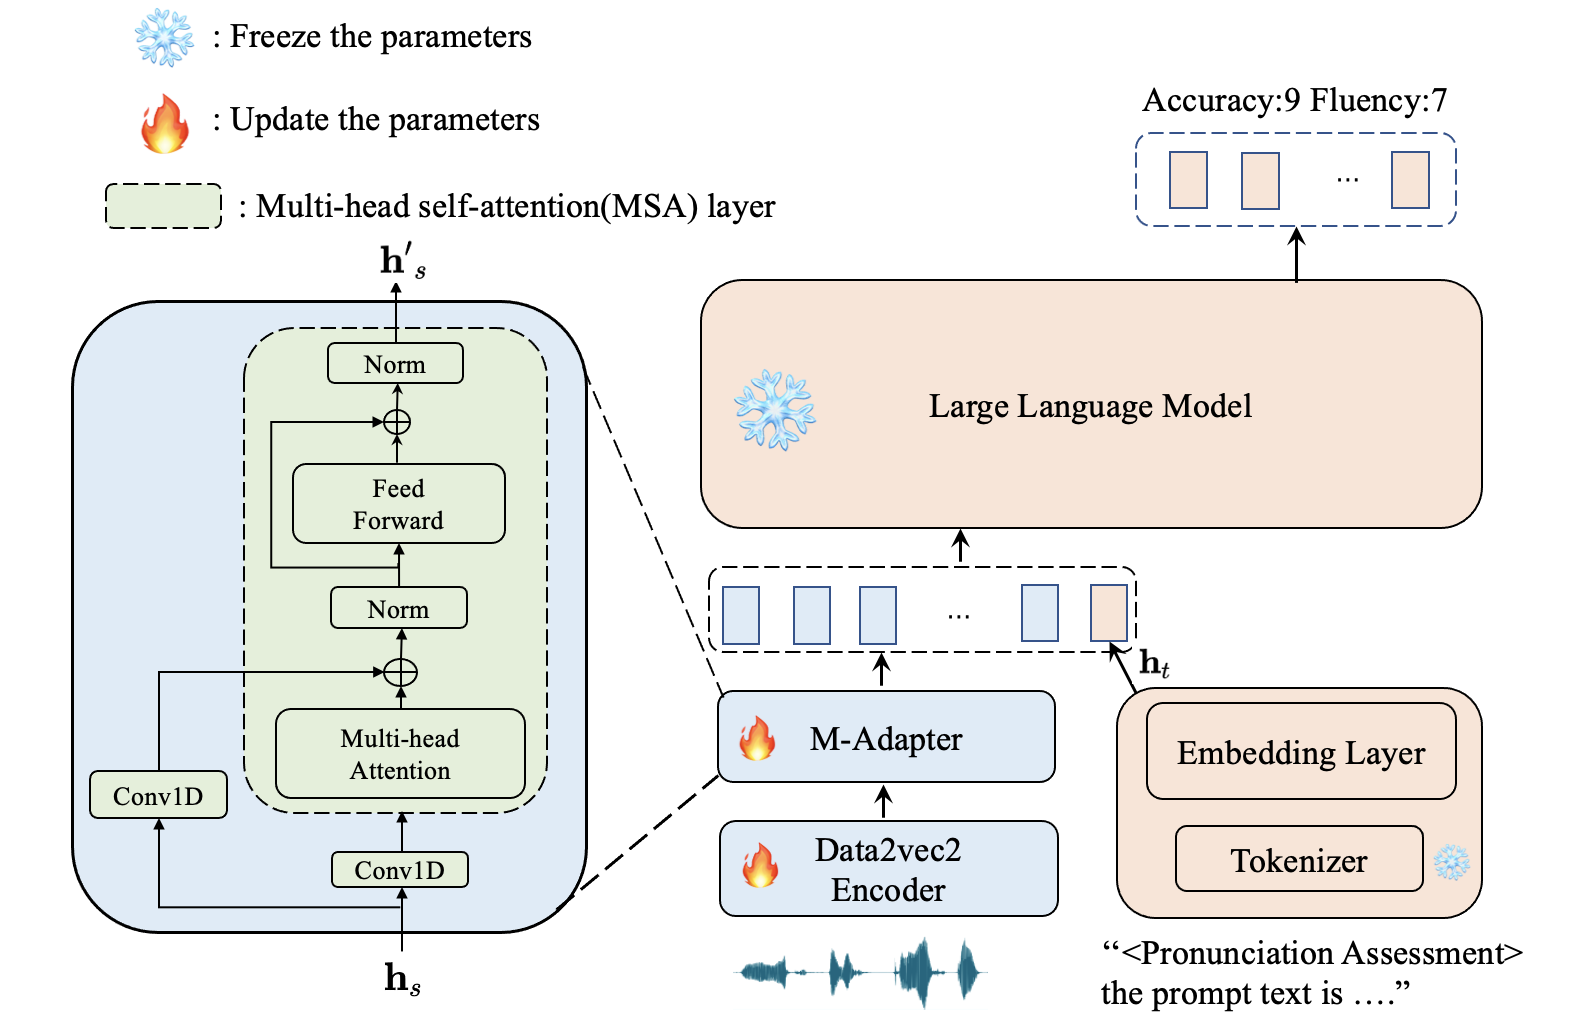
\includegraphics[width=0.6\textwidth]{content/figs/model7.png}
\caption{The overall pipeline for L2 learner's pronunciation assessment in the proposed system.}
\label{fig: model}
\end{figure*}

\begin{itemize}
    \item To our knowledge, this paper is the first to use a multi-modality model based on the LLM for pronunciation assessment. 
    \item The proposed multi-modal method belongs to the align-free system category and has achieved competitive performance compared to traditional align-based and align-free systems, which also verifies the effectiveness of this method.
    \item We contributed to a multi-modal system that achieved state-of-the-art (SOTA) results in ASR when we finished the training in the first stage.
\end{itemize}



\section{Proposed Method}
This section describes the proposed multi-modal pronunciation assessment method. First, we outline the three components of our system: the pre-trained acoustic encoder from data2vec2, the m-adapter as a modality adapter, and the LLM-based pronunciation assessment module. Then, we introduce the two-stage training process. The overall pipeline for pronunciation assessment is illustrated in Figure~\ref{fig: model}. 

\subsection{Speech Encoder}
Data2vec2~\cite{data2vec2} was employed as the audio encoder because of its versatility, efficiency, and outstanding performance in speech tasks. It comprises several convolutional blocks and multi-layer transformers. The convolutions in each block have 512 channels with strides of (5, 2, 2, 2, 2, 2, 2) and kernel sizes of (10, 3, 3, 3, 3, 2, 2). It transforms 16 kHz raw audio into a sequence of embeddings with a stride of 20 ms and a receptive field of 25 ms.

For each sample, given the raw audio $\mathbf{x_s}$, the speech features $\mathbf{h_s}$ was firstly extracted from the last hidden layer through the data2vec2 based speech encoder, which can be written as:

\begin{equation}
\label{eq:speech_encoder}
\mathbf{h_s} =  {SpeechEncoder}(\mathbf{x_s}),
\end{equation}


\subsection{Modality adapter}
The m-adapter~\cite{m-adapter} was firstly introduced for speech translation tasks. We employed it as a modality adapter in our model to connect the speech and text modalities. It consists of two pooling convolutions and a multi-head self-attention (MSA) layer. The pooling operations are used to modify the speech sequence length, while the MSA captures global information.

This work follows the paper~\cite{seamless} by replacing the three independent pooling modules for Q, K, and V with a shared pooling module to streamline the architecture and improve the efficiency of the model. In general, given the speech features $\mathbf{h_s}$ extracted from the speech encoder, a convolutional pooling operation is first used to adapt the speech length. These adapted features are then fed into the MSA layers to obtain the modality adapter features $\mathbf{{h'}_s}$, expressed as follow:

\begin{equation}
\label{eq:adapter}
\mathbf{{h'}_s} =  {Adapter}(\mathbf{h_s}),
\end{equation}

% 这个模块的直觉是，语音信号在时域上的特征数量比文本长度要大得多，一种scale的方法需要被应用在语音特征上来平衡两个模态的信息量。
The intuition of this module is that the number of features in the time domain of the speech signal is much larger than the length of the text. A scaling method needs to be applied to the speech features to balance the amount of information between the two modalities.

\begin{table*}[t!]
\vspace{1pt}
  \centering
  \caption{The WER results on Librispeech dataset comparing with other multi-modal systems. We briefly outlined the differences in these systems regarding speech encoders and modality adapters. Extra data indicates that these systems used additional training data besides Librespeech.}
   \label{table:asr_main}
\begin{tabular}{llcccc}
\toprule
      \multicolumn{1}{l}{\textbf{Model}}       & \textbf{Speech encoder} & \textbf{Modality adapter}    & \textbf{Extra data}  & \textbf{Test-clean} & \textbf{Test-other}   \\ \midrule
      SALMONN \cite{salmonn}           &    Whisper~\cite{whisper}, Beats   &  Q-former     &   \cmark             & 2.4                 & 5.4                        \\
      WavLLM~\cite{wavllm}     &  Whisper, WavLM          &  Linear &  \cmark         & 2              &  4.8                         \\  
      Qwen-Audio \cite{qwen_audio}  &  Whisper    & Linear &    \cmark   &   2.04     &  4.19                        \\ 
     SALM \cite{salm}  &     Hubert~\cite{hubert}   &  Linear &  \xmark       &   1.94        & 3.81                       \\ 
     Proposed   &     Data2vec2   & M-adapter & \xmark       &   \textbf{1.73}          &  \textbf{3.7}                       \\ 

\bottomrule

\end{tabular}
\end{table*}

\subsection{Pronunciation assessment with LLM}
Decoder-only LLM serves as a foundational component in the proposed method. We expect it to understand the learner's speech, analyse the difference between speech and the canonical text, and then make decisions regarding accuracy and fluency scores accordingly. 

For the text input of the LLM, we define the task-specific prefix as ``$<Pronunciation~Assessment>$". Additionally, in follow-up scenarios, The prompt text, as an important reference cue, can be considered as the text input of the LLM. Therefore, the final text input of LLM is defined as ``$<Pronunciation~Assessment> the~prompt~text~is~...$", and then the text input will be transformed into embedding features denoted as $\mathbf{{h}_t}$. Finally, we concatenate the embedding features with adapter-modified speech features $\mathbf{{h'}_s}$ and then fed the concatenated features into the LLM to obtain the final prediction text $\mathbf{y}$ through a token decoding operation as equation\eqref{eq:llm}, where the [;] denotes the concatenation of two vectors.


\begin{equation}
\label{eq:llm}
\mathbf{y} =  {LLM}([\mathbf{{h'}_s};\mathbf{h_t}]),
\end{equation}

\subsection{Two stages training  strategy}
The proposed method adopts a two-stage training strategy. Previous studies have shown that the performance of traditional align-based methods can be affected by the ASR system, as accuracy scoring heavily relies on speech content recognition. Therefore, in the first stage, we train the multi-modal model on the ASR task to make the connection between the two modalities more robust, which may benefit the pronunciation assessment task. We took the ASR task-specific prefix ``$<transcript>$" as the text input and then utilized limited ASR data to complete the ASR task training.

In the second stage, we fine-tuned the model trained in the first stage using a limited amount of scoring data based on the ``$<pronunciation~assessment>$" assessment task-specific prefix and prompt text. For the ground truth, we structured it as ``$accuracy:9~fluency:7$", aiming for LLM to output scores in such a format to achieve multi-task scoring for both accuracy and fluency. 



\section{Experimental setup}

\subsection{Datasets}
Two public datasets were used in this study. Librispeech~\cite{librispeech}, a commonly used ASR corpus, was utilized to train the multi-modal ASR in the first stage. It consists of about 1,000 hours of 16kHz read English speech derived from read audiobooks, with the dev-clean and dev-other subsets used as the validation set, and the test-clean and test-other subsets used as the test sets. To evaluate fluency and accuracy scoring in the second stage, we conducted experiments on Speechocean762~\cite{speechocean}, an open-source speech assessment corpus consisting of 5,000 English utterances collected from 250 Chinese speakers. The whole scoring dataset is divided into 2,500 sentences for training and 2, 500 for testing. The score distribution of the test set is shown in Figure 2. The x-axis represents the human-labeled scores, and the y-axis represents the number of occurrences for each corresponding score. % 补充内容说是classess


\begin{figure}[t!]
\centering
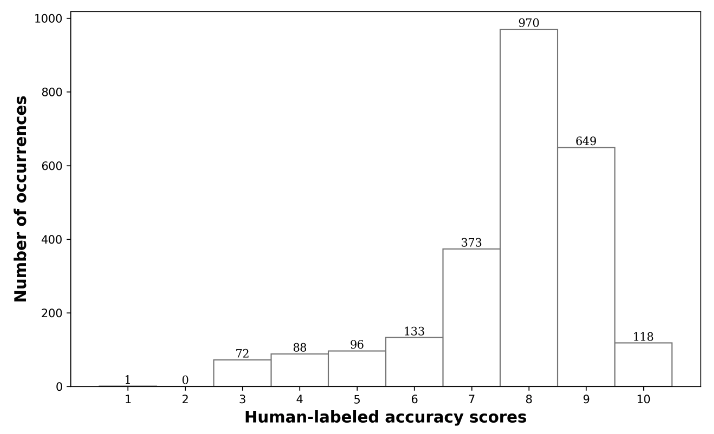
\includegraphics[width=0.35\textwidth]{content/figs/acc3.png}
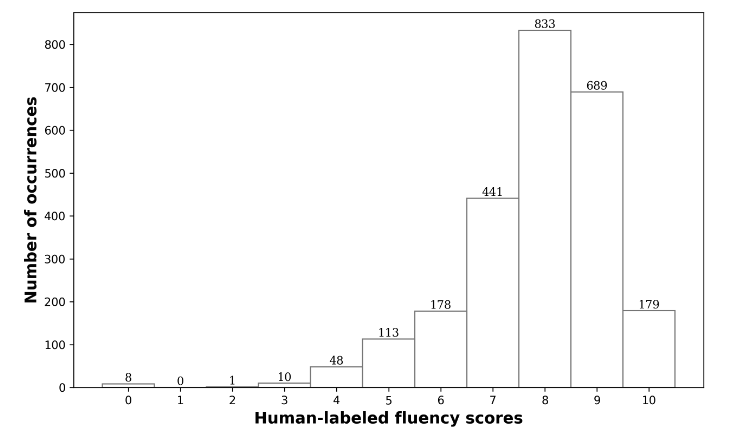
\includegraphics[width=0.35\textwidth]{content/figs/flu1.png}
\caption{The distribution of the human-labeled scores}
\label{fig: model}
\end{figure}

% \begin{figure}[t!]
% \centering
% \includegraphics[width=0.5\textwidth]{acc2.png}
% \caption{The overall pipeline for L2 learner's pronunciation assessment in the proposed system.}
% \label{fig: model}
% \end{figure}


\subsection{Setup}


% TODO
The weight of the data2vec2-based speech encoder is initialized from data2vec2-large~\footnote{\scriptsize{https://dl.fbaipublicfiles.com/fairseq/data2vec2/large\_vox\_960h.pt}} and the Qwen-based LLM~\cite{qwen} is initialized using pre-trained weights derived from Qwen-7B~\footnote{\scriptsize{https://huggingface.co/Qwen/Qwen-7B}}. For the M-adapter, we chose one MSA layer with 16 heads. The kernel size and stride of the convolution were both set to 2, aiming to halve the length of speech features extracted from the speech encoder.  

We used 8 A800s for the experiments. Each stage was trained for a maximum of two epochs on the corresponding task data. The ASR and pronunciation scoring training took about 9 and 0.2 hours, respectively. During both stages, the parameters of LLM were frozen, and the parameters of the speech encoder and modality adapter were updated. 



\section{Results and Discussion}
This section first presents the ASR result of the proposed system from the first training stage. Then, we demonstrate the pronunciation assessment results after fine-tuning the model based on the ASR training. Additionally, we present ablation experiments to explore the impacts of ASR training and prompt text. The scoring system performance was evaluated using the Pearson correlation coefficient (PCC) between the predicted scores and the human-labeled scores.




\subsection{Performance of ASR}
ASR task was often used to evaluate the performance of multi-modal systems\cite{salmonn,wavllm,qwen_audio,salm}. In this subsection, we selected several representative multi-modal systems with strong ASR performance as our baselines, including SALMONN~\cite{salmonn}, WavLLM~\cite{wavllm}, Qwen-Audio~\cite{qwen_audio}, and SALM~\cite{salm}. 

\begin{table*}[t!]
\vspace{1pt}
  \centering
  \caption{The PCC results on Speechocean762 dataset comparing with other baseline systems.}
   \label{table:main_result}
\begin{tabular}{llcccc}
\toprule
      \multicolumn{1}{l}{\textbf{Type}}   & \textbf{Methods}    & \textbf{Fluency} & \textbf{Accuracy}     \\ \midrule
       \multirow{3}{*}{Align-based}  &   GOPT~\cite{gopt}           &    0.753   &  0.714                        \\
                                    &    Multi-task~\cite{wong22_interspeech}      &  0.73          &  0.694                 \\  
                                    &   MultiPA~\cite{multipa}  &  0.772    & 0.705           \\   
                                    &   HiPAMA \cite{hipama}  &  0.762    & 0.730           \\   \midrule
       \multirow{3}{*}{Align-free}   & SSL~\cite{ssl1}  &     0.78   &  -          \\ 
                                     & SSL+IDX~\cite{liuwei}  &     0.795   &  -          \\ 
                                    &  \textbf{Proposed}   &     \textbf{0.777}   & \textbf{0.713}                 \\ 

\bottomrule

\end{tabular}
\end{table*}



\begin{table}[ht]
  \centering
  \caption{The WER results of speech encoder models in the proposed method.}
   \label{table:asr1}
\begin{tabular}{clcccc}
\toprule
      \multicolumn{1}{l}{\textbf{Method}}   & \textbf{Speech encoder}  & \textbf{Test-clean} & \textbf{Test-other}   \\  
   \midrule
   \multirow{3}{*}{Proposed}  &  Whisper        & 2.28              & 6.34                 \\
                              &  Hubert       & 1.83             &  \textbf{3.68}                \\ 
                              &  \textbf{Data2vec2}      & \textbf{1.73}              & 3.7                 \\ 
                              
\bottomrule
\end{tabular}
\end{table}


The comparison results between the proposed system and these baseline systems are shown in Table~\ref{table:asr_main}. For the result of the proposed method, the predict and ground-truth texts were normalized using Whisper's text normalization method~\footnote{\scriptsize{https://github.com/openai/whisper/tree/main/whisper/normalizers}} before computing WER. The results suggest that the proposed method outperforms all the baselines in terms of WER in the Librispeech test sets. This observation encourages us greatly for our upcoming pronunciation assessment tasks.

In addition, we briefly compared several different speech encoders based on the proposed method, with results shown in Table~\ref{table:asr1}. The findings reveal that the data2vec2 model as the optimal choice for speech encoding performs significantly better compared to the performance of Hubert~\footnote{\scriptsize{https://huggingface.co/facebook/hubert-large-ls960-ft}} and Whisper~\footnote{\scriptsize{https://huggingface.co/openai/whisper-large-v2}}.


%此外我们简单的对比了几种不同的speech encoder基于提出的方法，结果如表2所示。结果显示只针对英语语音训练的自监督模型在多模态上微调后的表现要显著好于多语种训练的whisper模型，并且data2vec2作为语音编码器取得了最优的效果。

\subsection{Results of pronunciation assessment}
In this subsection, we present the performance of the proposed multi-modal model in pronunciation scoring, which is an align-free end-to-end approach. For a fair comparison, we selected two types of baseline systems: one is align-free end-to-end systems based on SSL features and the other one is align-based systems that rely on traditional DNN-HMM based ASR model trained with Librispeech dataset. We did not consider the align-based system using SSL features~\cite{3m} as our baseline, since such an approach would make the entire align-based pipeline more complicated and less feasible for practical implementation.

We first conducted performance comparisons between the proposed multi-modal pronunciation scoring system and the align-based baseline systems presented in Table~\ref{table:main_result}. The leading results validate the effectiveness of our proposed method.
Moreover, compared to the complex pipelines of align-based systems, our proposed method offers a simpler way to evaluate learners' pronunciation. 

Then, we evaluate the performance comparisons with the align-free methods. The proposed method demonstrates competitive results with baseline systems in fluency scoring. Additionally, it fills the gap in accuracy scoring for align-free approaches on the Speechocean762 dataset.




%Figure 6.6 shows that the proposed scoring model can differentiate between lower levels of proficiency, but we can clearly see that it is not able to discriminate between the highest levels, 





%尽管先前有研究[]表示在该数据集上展现了更好的结果，但是该系统比较复杂，由DNN-HMM based system，SSL feature extractor model model and a scoring model 组成，很难


\subsection{Ablation studies}
In this subsection, we conducted experiments to determine the relative importance of ASR training in the first stage and prompt text in the proposed system for pronunciation scoring. The results are presented in Table~\ref{table:ablation}.

Firstly, we can clearly see that these two factors slightly improve fluency scoring performance in system (a). The two factors focus more on the content of the speech. As verified in \cite{our1,our2}, prosodic information is more important than speech content information for fluency scoring. Moreover, compared to SSL system~\cite{ssl1}, SSL+IDX~\cite{liuwei}showed a slight performance difference due to the additional information provided by phoneme IDs, which represent speech content. This further confirms that the content does not have a significant impact on fluency scoring.

Compared to speech fluency, accuracy is more significantly affected by these factors. The results of systems (b) and (c) show that the impact of introducing the prompt text is greater than that of ASR training. Additionally, system (d) found that not using any strategies resulted in poor accuracy scoring performance.

\begin{table}[ht]
\vspace{1pt}
  \centering
  \caption{The PCC results of ablation studies for the proposed method.}
   \label{table:ablation}
\begin{tabular}{llcccc}
\toprule
            &      \textbf{Factors}    & \textbf{Fluency} & \textbf{Accuracy}     \\ \midrule
       (a) & ASR training + Prompt text   &      \textbf{0.777}          &  \textbf{0.713}                 \\  
      (b) &         ASR training only      &   0.763    & 0.698           \\   
      (c) &          Prompt text only     &   0.768    & 0.665          \\  
      (d) &                      -      &    0.759    & 0.654          \\  

\bottomrule

\end{tabular}
\end{table}












\section{Conclusions}
This paper introduces the multi-modal approach to develop an end-to-end pronunciation assessment system for scoring fluency and accuracy of learners' L2 speech, such that it does not require any word and phone-level alignment information as input. The experiment results show that our approach achieves a competitive performance compared with previous methods, including those systems that utilize alignment information. This work can be used as the baseline system of end-to-end multi-modal approach and align-free related approach for pronunciation assessment tasks. Additionally, our proposed method achieved state-of-the-art (SOTA) performance in the ASR task, demonstrating the superior effectiveness of our multi-modal system. 

In the future, we will investigate the chain-of-thought (COT)~\cite{cot} ability of the proposed system to provide step-by-step explanations for the model's scoring decisions.

%\bibliographystyle{style/IEEEbib}
\bibliographystyle{IEEEbib}
%\bibliography{strings,refs}
%\bibliography{strings,refs}

\small
\bibliography{strings,main}

\end{document}
